\chapter{Random Testing}
\label{chap:randomTesting}

%\section{Random Testing}
%This text is blue because we have to change it to our own words

\textcolor{blue}{Work on random test generation dates back to a 1970 paper by Hanford. In it he reports on the ``syntax machine", a program that generated random but syntactically-correct programs for testing PL/I compilers \cite{hanford1970automatic}. The next published work on random testing was a 1983 paper by Bird and Munoz \cite{bird1983automatic}. They describe a technique to
generate randomly-generated ``self-checking" test cases: test cases that in addition to generating test inputs generated checks for expected outputs using knowledge of the semantics of the software under test. For example, when generating random programs for testing a compiler, the generator kept track of the expected values of arithmetic computations and inserted the appropriate checks into the test case. They also applied their technique to checking sorting and merging procedures and graphic display software~\cite{pacheco2009directed}.}


Random testing is a dynamic black-box testing technique in which the software is tested with non-correlating or unpredictable test data from the specified input domain~\cite{Chan2002}. The input domain is a set of all possible inputs to the software under test. According to Richard~\cite{hamlet1994}, in random testing, input domain is first identified, then test points are randomly taken from the whole input domain by means of random number generator. The program under test is executed on these points and the results obtained are compared with the program specifications. The test fails if the results are not according to the specifications and vice versa. Failure of any test results reflects error in the SUT.

\begin{figure}[h]
	\centering
	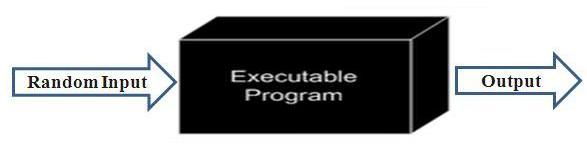
\includegraphics[scale=0.5]{chapter3/randomTesting.jpg}
	\caption{Random Testing}
\end{figure}

Generating test data by random generator is quite economical and requires less intellectual and computational efforts~\cite{Ciupa2008a}. Moreover, no human intervention is involved in data generation that ensures an unbiased testing process.

However, generating test cases with out using any background information makes random testing susceptible to criticism. It is criticized for generating many test cases ending up at the same state of software. It is further stated that, random testing generates test inputs that violates requirements of the given SUT making it less effective~\cite{pacheco2009directed, sen2007effective}. Myers mentioned random testing as one of the least effective testing technique~\cite{Myers1979}.

It is stated by Ciupa et al. \cite{Ciupa2007}, that Myers statement was not based on any experimental evidence. Later experiments performed by several researchers~\cite{hamlet1994, Ciupa2008, leitner2007efficient, Duran1981} confirmed that random testing is as effective as any other testing technique. It was found experimentally~\cite{Duran1981} that random testing can also discover subtle faults in a given SUT when subjected to large number of test cases. It was pointed out that the simplicity and cost effectiveness of random testing makes it more feasible to run large number of test cases as opposed to systematic testing techniques which require considerable time and resources for test case generation and execution. The empirical comparison proves that random testing and partition testing are equally effective~\cite{hamlet1990}. A comparative study conducted by Ntafos~\cite{ntafos1998random} concluded that random testing is more effective as compared to proportional partition testing.

\textcolor{blue}{One of the best-known works in the field is Miller et al.’s “fuzz testing” paper, where they generate random ASCII character streams and use them as input to test Unix utilities for abnormal termination or non-terminating behaviour \cite{miller1990empirical}. In subsequent work, they extended fuzz testing to generate sequences of keyboard and mouse events, and found errors in applications running in X Windows, Windows NT and Mac OS X \cite{forrester2000empirical, miller2006empirical}. Today, fuzz testing is used routinely in industry. It is frequently used as a tool for finding security vulnerabilities and is applied to test formats and protocols that attackers might use to gain unauthorized access to computers over a network. Other work that applies random test generation to operating systems code includes Kropp’s use of random test generation to test low-level system calls \cite{kropp1998automated}, and Groce et al.’s use of random test generation at NASA to test a file system used in space missions \cite{groce2007randomized}. In all these studies, a random test generator invariable found many errors in the software under test, and many errors were critical in nature. For example, Groce et al. found dozens of errors in the file system under test, many of which could have jeopardized the success of a mission.}

\section{Various versions of random testing}
Researchers have tried various approaches to bring about improvement in the performance of random testing. The prominent modifications in random strategy are stated below:

\subsection{Adaptive Random Testing}
Adaptive random testing (ART), proposed by Chen et al.~\cite{Chen2008} is based on the previous work of Chan et al.~\cite{Chan1996} regarding the existence of failure patterns across the input domain. Chan et al. observed that failure inducing inputs in the whole input domain form certain geometrical patterns and divided these into point, block and strip patterns described below.

\begin{enumerate}
\item {\bf Point pattern:} In the point pattern inputs inducing failures are scattered across the input domain in the form of stand-alone points. Example of point pattern is the division by zero in a statement {\it total = num1/num2;} where {\it num1}, {\it num2} and {\it total} are variables of type integer.
\item {\bf Block pattern:} In the block pattern inputs inducing failures lie in close vicinity to form a block in the input domain. Example of block pattern is failure caused by the statement {\it if ( (num \textgreater 10) \&\& (num \textless 20) )}. Here 11 to 19 are a block of faults.
\item {\bf Strip pattern:} In the strip pattern inputs inducing failures form a strip across the input domain. Example of strip pattern is failure caused by a statement {\it num1 + num2 = 20}. Here multiple values of {\it num1} and {\it num2} can lead to the fault value 20. 
\end{enumerate}

\begin{figure}[h]
	\centering
	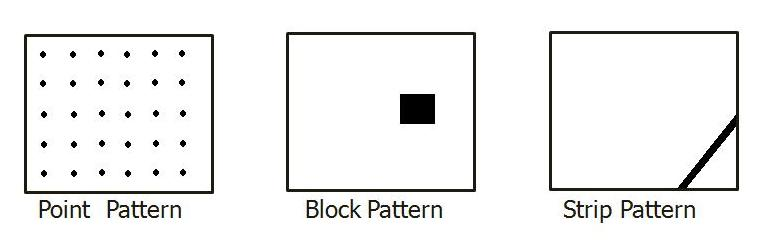
\includegraphics[scale=0.5]{chapter3/pointblockstrip.jpg}
	\caption{Patterns of failure causing inputs}
	\label{fig:patterns2}
\end{figure}

In figure~\ref{fig:patterns2} the square boxes indicate the whole input domains. The white space in each box shows legitimate and faultless values while the black colour in the form of points, block and strip inside the respective box indicates the point, block and strip fault patterns.

Chen et al. ~\cite{Chen2008} argued that ordinary random testing might generate test inputs lurking too close or too far from the input inducing failure and thus fails to discover the fault. To generate more faults targeted test inputs, they proposed Adaptive Random Testing (ART) as a modified version of ordinary random testing where test values are selected at random as usual but are evenly spread across the input domain by using two sets. The executed set comprises the test cases executed by the system and the candidate set includes the test cases to be executed by the system. Initially both the sets are empty. The first test case is selected at random from the candidate set and stored in executed set after execution. The second test case is then selected from the candidate set which is far away from the last executed test case. In this way the whole input domain is tested with greater chances of generating test input from the existing fault patterns.

In the experiments conducted by Chen et al.~\cite{Chen2008} the number of test cases required to detect first fault (F-measure) was used as a performance matrix instead of the traditional matrix P-measure and E-measure. Experimental results using ART showed up to 50\% increase in performance compared to ordinary random testing. The authors admitted that the issues of increase overhead, spreading test cases across the input domain for complex objects and efficient ways of selecting candidate test cases still exist. Chen et al. continued their work on ART to address some of these issues and proposed its upgraded version in~\cite{chen2009enhanced} and~\cite{Chen2005}. 

\subsection{Mirror Adaptive Random Testing}
%As discussed in the above section ART provide better results, however the increase in overhead due to extra computation to achieve even spread of test inputs makes it less cost effective. 
Mirror Adaptive Random Testing (MART)~\cite{Chen2003} is an improvement on ART by using mirror-partitioning technique to decrease the extra computation involved in ART and reduce the overhead.

\begin{figure}[h]
\begin{center}
	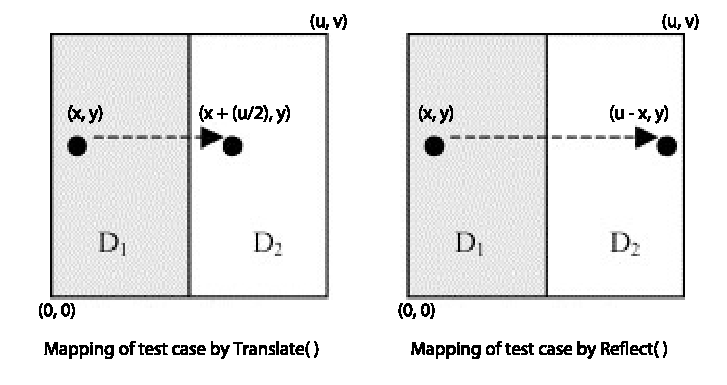
\includegraphics[width=13cm, height=6cm ]{chapter3/mart2.pdf}
	\caption{Mirror Adaptive Random Testing~\cite{Chen2003}}
\label{fig:mirrorART}
\end{center}  
\end{figure}

In this technique, the input domain of the program under test is divided into n disjoint sub-domains of equal size and shape. One of the sub-domains is called source sub-domain while all the others are termed as mirror sub-domains. ART is then applied only to the source sub-domain to select the test cases while from all other sub-domains test cases are selected by using mirror function. In MART {(0, 0), (u, v)} are used to represent the whole input domain where (0, 0) is the leftmost and (u, v) is the rightmost top corner of the two dimensional rectangle. On splitting it into two sub-domains we get {(0, 0), (u/2, v)} as source sub-domain and {(u/2, 0), (u, v)} as mirror sub-domain. Let suppose we get x and y test cases by applying ART to source sub-domain, now we can linearly translate these test cases to achieve the mirrored effect, i.e. (x + (u/2), y) as shown in the figure~\ref{fig:mirrorART}. Comparative study of MART with ART provide evidence of equally good results of the two strategies with MART having the added advantage of using only one quarter of the calculation as compared with ART and thereby reduces the overhead.


\subsection{Restricted Random Testing}
Restricted Random Testing~\cite{chan2003normalized} is another approach to overcome the problem of extra overhead in ART. Restricted Random Testing (RRT) achieves this by creating a circular exclusion zone around the executed test case. A candidate is randomly selected from the input domain for the next test case. Before execution the candidate is checked and discarded if it lies inside the exclusion zone. This process repeats until a candidate laying outside the exclusion zone is selected. This ensures that the test case to be executed is well apart from the last executed test case. The radius of exclusion zone is constant around each test case and the area of each zone decreases with successive cases.

\begin{figure}[h]
	\centering
	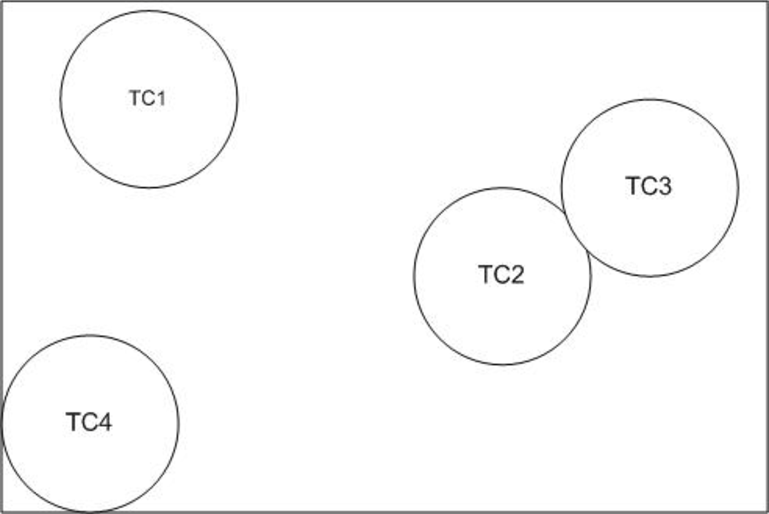
\includegraphics[width= 6cm, height = 5cm]{chapter3/RRT.pdf}
	\caption{Input domain with exclusion zone around the selected test case}
\end{figure}

To find the effectiveness of RRT, the authors compared it with ART and RT on 7 out of the 12 programs evaluated by ART and MART. The experimental results showed that the performance of RRT increases with the increase in the size of the exclusion zone and reaches the maximum level when the exclusion zone is raised to largest possible size. %Normalized Restricted Random Testing~\cite{chan2003normalized} is an improvement over RRT by allowing the testers to have better information about the target exclusion rate (R) of RRT. 
They further found that RRT is up to 55\% more effective than ordinary random testing in terms of F-measure (Where F-measure is the total number of test cases required to find the first failure).



\subsection{Directed Automated Random Testing}
Godefroid et al.~\cite{Godefroid2005} proposed Directed Automated Random Testing (DART). %Its main purpose was to overcome the cost and difficulty of manual testing while keeping its quality intact. It automate the whole testing process including generation of unit tests, test drivers/harness and assertions for functional correctness. 
The main features of DART can be divided into the following three parts:
\begin{enumerate}
\item {\bf Automated Interface Extraction:} DART automatically identifies external interfaces of a given SUT. These interfaces include external variables, external functions and the user-specified main function, which initializes the program execution.
\item {\bf Automatic Test Driver:} DART generate test drivers to run the test cases. All the test cases are randomly generated according to the underlying environment.
\item {\bf Dynamic Analysis of execution:} The DART instruments the given SUT at the start of the process in order to track its behaviour dynamically at run time. The results obtained are analysed in real time to systematically direct the test case execution along alternative path for maximum code coverage.
\end{enumerate}

The DART algorithm is implemented in the tool which is completely automatic and accepts the test program as input. After the external interfaces are extracted it then use the pre-conditions and post-conditions of the program under test to validate the test inputs. For languages that do not support contracts inside the code (like C), they used public methods or interfaces to mimic the scenario -------- to be continued

\subsection{Quasi Random Testing}
Quasi-random testing (QRT)~\cite{Chen2005} is a testing technique which takes advantage of failure region contiguity by distributing test cases evenly with decreased computation. %Chan et al after the analysis of faults in various experiments found that the fault patterns across the input domain are continuous. 
To achieve even spreading of test cases, QRT uses a class with a formula, that forms an s-dimensional cube in s-dimensional input domain and generates a set of numbers with small discrepancy and low dispersion. The set of numbers is then used to generate random test cases that are permuted to make them less clustered and more evenly distributed. An empirical study was conducted to compare the effectiveness of QRT with ART and RT. The empirical results of the experiments showed that in 9 out of 12 programs QRT found a fault quicker than ART and RT while there was no significant improvement in the remaining three programs.
%\subsection{Monti Carlo Random Testing}

%\subsection{Good Random Testing}

\subsection{Feedback-directed Random Testing}
Feedback-directed Random Testing (FDRT)~\cite{Pacheco2007} is a technique that generate unit test suite at random for object-oriented programs. As the name implies FDRT uses the feedback received from the execution of first batch of randomly selected unit test suite to generate next batch of more directed unit test suite. In this way redundant and illegal unit tests are eliminated incrementally from the test suite with the help of filtration and application of contracts. For example unit test that produce IllegalArgumentException on execution is discarded, because, selected argument used in this test was not according to the type of argument the method required. 

%\subsection{Adaptive Random Testing for Object-Oriented}
\subsection{The ARTOO Testing}
The Adaptive Random Testing for Object Oriented (ARTOO) strategy is based on object distance. Ciupa et al.~\cite{Ciupa2006}, defined the parameters that can be used to calculate distance between the objects. Two objects have more distance between them if they have more dissimilar properties. The parameters to specify the distance between the objects are dynamic types and values assigned to the primitive and reference fields. Strings are treated in terms of directly usable values and Levenshtein formula~\cite{Levenshtein1966} is used as a distance criteria between the two strings.

In the ARTOO strategy, two sets are taken i.e. candidate-set containing the objects ready to be run by the system and the used-set, which is empty. First object is selected randomly from the candidate-set which is moved to used-set after execution. The second object selected from the candidate-set for execution is the one with the largest distance from the last executed object present in the used-set. The process continues till the bug is found or the objects in the candidate-set are finished~\cite{Ciupa2006}.

The ARTOO strategy, implemented in AutoTest tool \cite{Ciupa2008a}, was evaluated in comparison with Directed Random (D-RAN) strategy by selecting classes from EiffelBase library \cite{meyer1987eiffel}. The experimental results indicated that some bugs found by the ARTOO were not identified by the D-RAN strategy. Moreover the ARTOO found first bug with small number of test cases than the D-RAN strategy. However, computation to select test case in the ARTOO strategy was more than the D-RAN strategy thus it took more time to generate a test case.

% the same team implemented that model and performed several experiments to evaluate the proposed model. Adaptive Random Testing for Object Oriented (ARTOO) is a testing strategy, based on object distance, implemented in AutoTest tool \cite{16 search it Mendeley}.
%ARTOO was implemented as a plug-in strategy in AutoTest. It only deals with creating and selecting inputs and all other functionality of the AutoTest was the same. Since ARTOO is based on object distance therefore the method for test input selection is to pick that object from the candidate set (A pool of objects that is a potential candidate to be executed by the system) that has the highest average distance in comparison to the objects already executed. In the experiments classes from EiffelBase library \cite{17 search it mendeley} were used. To evaluate ARTOO the same tests were also applied to directed random strategy (RAND). The outcome of the experiments showed that ARTOO finds the first bug with fewer test cases than RAND. The computation to select test case in ARTOO is more than RAND and therefore ARTOO takes more time to generate a test input. The experiments also found few of the bug found by ARTOO were not pointed out by RAND furthermore ARTOO is less sensitive to the variation of seed value than RAND
. 
%\subsection{Object Distance and its application}
%To improve the performance of random testing the emphasis of ART was on the distance be- tween the test cases. But this distance was defined only for primitive data types like integers and other elementary input. Ciupa et al defined the parameters that can be used to calculate distance between the composite programmer-defined types so that ART can be applicable to testing of today’s object-oriented programs~\cite{Ciupa2006}. Two objects have more distance between them if they have more dissimilar properties. The parameters to specify the distance between the objects are dynamic types, values of its primitive and reference fields. Strings are treated as a directly usable values and Levenshtein distance~\cite{Levenshtein1966} that is also known as edit distance is used as a distance criteria between the two strings. To implement object distance first all the distances of the objects are measured. Then two sets candidate- objects containing the all the objects ready to be run by the system and the used-objects set, which is initially empty. First object is selected randomly from the candidate-object set and is moved to used-object set when executed by the system. Now the second object selected from the candidate set for execution is the one with the biggest distance from the last executed object present in the used-object set. This process is continuing until the bug is found or the objects in the candidate-object set are finished.

%\subsubsection{Experimental Assessment of RT for Object-Oriented Software}
%In this research the effect of various parameters involved in random testing and its effect on efficiency is evaluated by performing various experiments on Industrial-grade code base. Large-scale clusters of computers were used for 1500 hours of CPU time which resulted in 1875 test sessions for 8 classes under test.~\cite{Ciupa2007} The finding of the experiments are 1. Version of random testing algorithm that is efficient for smaller testing timeout is equally efficient for higher testing timeouts. 2. The value of seed for random testing algorithm plays a vital role in finding the number of bugs in specific time. 3. Most of the bugs are found in the first few minutes of the testing sessions.



\subsection{Design by Contract}
% section taken from binding yeti with .net, check it out correct it.
\textcolor{blue}{Modern software development as it is well known has adopted the paradigm of Object Oriented (OO) Programming. The primary and most important reason for this evolution is the desire for better quality software and a more efficient way to bridge the gap between requirements and code.
Industrial use of OO confirmed the superiority of this approach over procedural
programming languages. However, so far no final approach has been generally accepted over a methodology on how to construct OO software in order to achieve one of the most important factors of quality, which is reliability or else robustness. As the work of Dr. Bertrand Meyer has shown \cite{meyer1992applying, meyer1988object} the decision on how to make software more reliable is crucial if the developers want to use the benefits of OO. These benefits include:
1 Reuse of software components. This implies using a software component at multiple environments apart from the environment in which its developers originally deployed it.
2 The goal of having reliability plays an important role in characterizing the quality of a software module.
3 The abstract types that OO introduces. A reliable way to construct abstract types emerges. To achieve the previous goals the software development world has used two approaches, Defensive programming and Design by Contract. As the next paragraphs show the latter one has been showing more advantages than the first one. That is why most researches on Automated Testing use design by contract as a requirement that the SUT must conform to, in order for their tool to find as many bugs as possible \cite{Leitner2007}.
The idea of Defensive Programming, which is inherited from the software development world prior to OO, is in general advising to ―… include as many checks as possible even if they are redundant \cite{meyer1992applying}. This concept is intuitively stating that having extra checking can never do harm especially if someone wants to protect the software from inexperienced users. This last concept unfortunately is not correct. This kind of approach puts more code inside the software and this contributes to greater complexity of the software, and complexity as Dr. Meyer has very correctly stated ―…is the single worst obstacle to software quality in general, and to reliability in particular \cite{meyer1992applying}. The reason is that this extra code is a source of things that might go wrong and so we must also check it, and so on to infinitum. The need for a more systematic approach is evident based on the concept that software elements are implementations of well-understood specifications by the developers and that is exactly what Design by Contract does. Design by Contract concept adopts the idea that any operation a routine of a software performs, should bind the caller of that routine to the routine itself. This binding provides specific obligations that each party has, along with benefits. Essentially the obligations of one part describe the benefits of the other part. These ideas apply to software routines (i.e. methods, functions of classes) via assertions that implement the binding, which is like a contract between two persons. These assertions are classified into pre-conditions, post-conditions and class invariants. Figure 2.1 which is a figure of the ―Applying Design by Contract article \cite{meyer1992applying}, illustrates the use of these assertions.

As anyone can understand from Figure ?? pre and post-conditions denote the idea that if the caller promises to invoke the routine with the pre-conditions holding, the routine guarantees the caller that it will return the system in a final state in which the post-conditions hold. Thus, the invoker knows nothing about how the routine reaches the final state but can depend on the results. This implies another thing, which is that the routine is responsible only for the cases where the pre- conditions hold. This means rejecting the whole concept of defensive programming because if something is an assertion in the pre-condition the routine does not have to handle it in its body/code and vice versa. Overall, it is forbidden for the same assertion to exist in both parts. How strong or weak a pre-condition should be is a decision of the developer. So far the notions of pre and post-conditions are assertions that developers can use even with procedural programming languages at each of their routines. The notion that enhances more the efficiency of the contracts is the notion of the class invariant. Through class invariants a developer can describe a general condition that any instantiation of that class must hold at any time \cite{meyer1992applying, meyer1988object}. By this the developers classify the requirements that they have in the same abstract way in which they develop the software; making the bridging of requirements to code more traceable, thus more possible to achieve all the requirements, the basic goal of software development.
In addition, to the previous benefits design by contract can facilitate documentation. By providing contract information documentation describes a module of code certainly better than just presenting the interface and the result it yields. Furthermore, monitoring these assertions can be very helpful while debugging.
It is up to the developers to decide what the software must do when one of the parties breaks a contract. It can stop the execution, prompt the event, ask the user to decide etc. It is a decision based on the specifications. Basically as the article of Meyer B. \cite{meyer1992applying} describes, three things can mainly occur
1. An alternative algorithm starts due to this exceptional behaviour 2. System stops its executions and returns to a prior consistent state 3. A rare but possible false alarm has happened due to operating system or hardware signals and after correcting actions execution continues
The general approach is to consider and to monitor any violation because most of the times this violation describes a bug. Either in the logic of the requirements (pre-conditions, class invariants) or in the algorithm of the implementation (post-conditions).
Sometimes research papers mention the contracts of the code as partial specifications \cite{daniel2007automated} because they provide more information than just requirements documents but at the same time they are not a full specification model which describes the whole algorithm of a software module as formal methods do.
Design by Contract principle helps developers use appropriately polymorphism and dynamic binding. With contracts, designers can have inheritance and reassure that the class that inherits another class will respect the original contract and if the designer wants he/she can add assertions based on the functionality of the child class. The rules that the designers must follow, to maximally use the contracts, is to allow the child classes, when it is desired, to: i) have weaker pre-conditions or ii) stronger post-conditions. In this way contracts provide an immediate guideline to the designer.}


%\section{Automated Random Testing Tools}
\section{Tools for Automated Random Testing}
A number of open-source and commercial random testing tools that automatically generate test cases, reported in the literature, are briefly described in the following section.


\subsection{JCrasher}
JCrasher is an automatic robustness testing tool developed by Csallner and Smaragadakis \cite{Pacheco2007b}. JCrasher tries to crash the Java program with random input and exceptions thrown during the process are recorded. The exceptions are then compared with the list of acceptable standards, defined in advance as heuristics. The undefined runtime exceptions are considered as errors. Since users interact with programs through its public methods with different kind of inputs, therefore, JCrasher is designed to test only the public methods of the SUT with random inputs.

\begin{figure}[h]
	\centering
	\includegraphics[width=15cm, height=7cm]{chapter3/JCrasher.png}
	\caption{Illustration of robustness testing of Java program with JCrasher~\cite{Pacheco2007b}}
	\label{fig:JCrasher}
\end{figure}

Figure~\ref{fig:JCrasher} illustrates the working of JCrasher by testing a {\it T.java} program. The source file is first compiled using {\it javac} and the byte code obtained is passed as input to JCrasher. The JCrasher, with the help of Java reflection~\cite{chan1999java}, analyse all the methods declared by class {\it T} using methods transitive parameter types { \it P} to generate the most appropriate test data set which is written to a file {\it TTest.java}. The file is compiled and executed by JUnit. All the exceptions produced during test case executions are collected and compared with robustness heuristic for any violation which is reported as error.\\

\noindent JCrasher is a pioneering tool with the capability to perform fully automatic testing, including test case generation, execution, filtration to report generation. JCrasher has the novelty to generate test cases as JUnit files which can also be easily read and used for regression testing. Another important feature of JCrasher is to execute each new test on a ``clean slate" ensuring that the changes made by the previous tests do not affect the new test.  

% check parameter space or parameter graph in the figure???


\subsection{Jartege}
Jartege (\uline{Ja}wa~\uline{r}andom~\uline{te}st~\uline{ge}nerator)~\cite{Oriat2004} is an automated testing tool that randomly generates unit tests for Java classes with contracts specified in Java Modelling Language (JML). The contracts include methods pre- and post-conditions and class invariants. Initially Jartege uses the contracts to eliminate irrelevant test cases and later on the same contracts serve as test oracle to differentiate between errors and false positives. Jartege uses simple random testing to test classes and generate test cases. In addition, it parametrise its random aspect in order to prioritise testing specific part of the class or to get interesting sequences of calls. The parameters include the following: 
\begin{itemize}
\item Operational profile of the classes i.e. the likely use of the class under test by other classes.  
\item Weight of the class and the method under test. Higher weight prioritizes the class or method over lower weight during test process. 
\item Probability of creating new objects during test process. Low probability means creation of fewer objects and more re-usability for different operations while high probability means numerous new objects with less re-usability.
\end{itemize}

\noindent The Jartege technique evaluates a class by entry pre-condition and internal pre-conditions. Entry pre-conditions are the contracts to be met by the generated test data for testing the method while internal pre-conditions are the contracts which are inside the methods and their violation are considered as error either in the method or in the specification. The Jartege checks for errors in program code as well as in specifications and the Junit tests produced by Jartege can be used later as regression tests. Its limitation is the requirement of prior existence of the program JML specifications.

\subsection{Eclat}
Eclat~\cite{Pacheco2005} is an automated testing tool which generates and classifies unit tests for Java classes. The process is accomplished in three main components. In the first component, it selects a small subset of test inputs, likely to reveal faults in the given SUT, from a large set.

\begin{figure}[h]
	\centering
	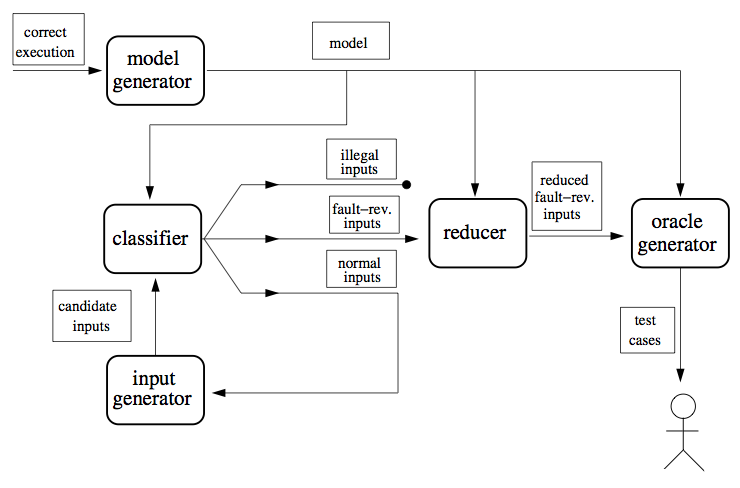
\includegraphics[width=15cm, height=9cm]{chapter3/eclat_working.png}
	\caption{Main component of Eclat contributing to generate test input~\cite{Pacheco2005}}
	\label{fig:eclat}
\end{figure}


\noindent The tool takes a software and a set of test cases for which the software runs properly. It then creates an operational model based on the correct software operations and apply the test data. If the operational pattern of execution of the test data differs from the model, the following three outcomes may be possible: (a) it sight a fault in the given SUT, (b) it might produce normal operations despite model violation, (c) it might be an illegal input that the program cannot handle. (note for author extend 2nd and 3rd component)
In the second component of the process, reducer function is used to discard any redundant input, leaving only a single input per operational pattern. In third component the acquired test inputs are converted into test cases, by creation of oracle, to determine the success or failure of the test. \\
\indent Eclat was compared with JCrasher by executing nine programs on  both tools individually~\cite{Pacheco2007b}. Based on the experimental results it was revealed that Eclat perform better than JCrasher. On the average, Eclat selected 5.0 inputs per run out of which 30\% revealed faults, while JCrasher selected 1.13 inputs per run out of which 0.92\% of those revealed faults. The limitation of Eclat is dependence on the initial pool of correct test cases and existence of any errors in the pool may lead to the creation of wrong operational model which will adversely affect the testing process.   

%\subsection{JTest}
%Parasoft Jtest is a commercial tool that automatically generates and execute unit tests. It can be easily integrated to Java IDEs like Eclipse where it provide two main functionalities, i.e. Static Analysis, Unit testing and code coverage. [25]
%In static analysis Jtest takes a complete project or set of classes as input and compares it with a list of built-in rules. The statement violating any of these rules is an error. It also suggests probable fixes for the detected fault.
%For unit testing it takes a class as an input and processes a number of scenarios against it to generate and execute unit tests. Once unit tests are executed they become the part of regression test for future reference.
%Jtest also shows the code coverage of the program by colour coding the statements that are not executed by the unit tests.


\subsection{Randoop Tool}
Random tester for Object Oriented Programs (RANDOOP) is the tool used for implementing FDRT technique~\cite{Pacheco2007b}. RANDOOP is a fully automatic tool, capable of testing Java classes and .Net binaries. It takes as input a set of classes, contracts, filters and time limit while its output is a suite of JUnit and NUnit for Java and .Net program respectively. Each unit test in a test suite is a sequence of method calls (hereafter referred as sequence). RANDOOP build the sequence incrementally by randomly selecting a public method from the class under test and arguments for these methods are selected from the predefined pool in case of primitive types and a sequence or null value in case of reference type. RANDOOP maintains two sets called ErrorSeqs and NonErrorSeqs to record the feedback. It extends ErrorSeqs set in case of contract or filter violation and NonErrorSeqs set when no violation is recorded in the feedback. The use of this dynamic feedback evaluation at runtime brings an object to very complex and interesting state. On test completion it produce ErrorSeqs and NonErrorSeqs as JUnit/NUnit test suite. In terms of coverage and number of faults discovered, RANDOOP implementing FDRT was compared with random testing of JCrasher and JavaPathFinder~\cite{visser2004test}. In their experiments, 14 libraries of both Java and .Net were evaluated. The results showed that RANDOOP achieved more coverage than JCrasher in behavioural, branch coverage and faults detection. It can achieve on par coverage with systematic approaches like JavaPathFinder. RANDOOP also has an edge over model checking for its ability to easily search large input domains.

\subsection{QuickCheck Tool}
QuickCheck~\cite{Claessen2000} is a lightweight random testing tool used for testing of Haskell programs~\cite{Hudak2007}. Haskell is a functional programming language where programs are evaluated by using expressions rather than statements as in imperative programming. In Haskell most of the functions are pure except the IO functions, thus main focus of the tool is on testing pure functions. These are the functions which depend on its input parameters and make changes to them only. QuickCheck tool is designed to have a simple domain-specific language of testable specifications embedded in Haskell. This language is used to define expected properties of the functions under test - for example, reversing a list with single element must result in the same list.\\ %(author check the definition of pure functions)\\
\indent The QuickCheck takes function to be tested and properties of the program defined by tester (Haskell functions) as input. The tool uses built-in random generator to generate effective test data, however, to get adequate coverage in the case of custom data types, the testers can also develop their own generator. On executing the function with test data, the tester defined properties must hold for the function to be correct. Any violation of the defined properties suggest error in the function.



% The function is executed against the generated test data. The QuickCheck evaluates and declares a fault in the function where a test case violates the set properties.   



%\subsection{AgitarOne}
%AgitarOne is a commercial tool that automatically generates unit tests. It has a Junit Generator engine that can create 25,000 lines or more of Junit per hour [29]. It can be easily integrated into famous IDE like Eclipse. It takes as input, classes under test, time and optionally any knowledge or test cases that has a positive influence on the performance of the testing process. The generated Junit tests can be run from the same IDE and can also be used for later regression testing. The GUI interface is called a dashboard which provides in depth knowledge of the tests conducted, failures detected, alerts and the archieves of the tests conducted earlier. It also shows the coverage obtained after executing the Junits against the code under test.

\subsection{Autotost Tool}
The Autotest tool, based on Formal Automated testing is used to test Eiffel language programs~\cite{Ciupa2007}. The Eiffel language uses the concept of contracts which is effectively utilized by Autotest - for example the auto generated input is filtered using pre-conditions and unwanted test input is discarded. The contracts are also used as test oracle to determine if the test is pass or fail. Beside automated testing the Autotest also allow the tester to manually write the test cases to target specific behaviour or section of the code. The Autotest scope can be a single method/class or cluster of methods/classes as inputs, it then automatically generate test input data according to the requirement of the methods or classes.

\begin{figure}[h]
	\centering
	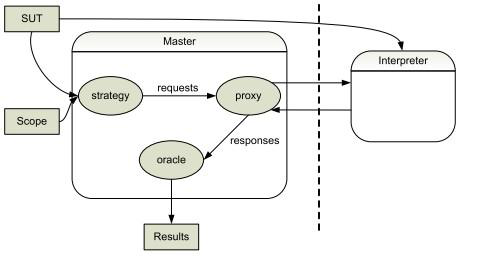
\includegraphics[width=13cm, height=7cm]{chapter3/autotest.png}
	\caption{Architecture of Autotest}
	\label{fig:autotest}
\end{figure}

\noindent According to Figure~\ref{fig:autotest}~\cite{Leitner2007}, the architecture of Autotest tool can be split into the following main parts:
\begin{enumerate}
\item \textbf{Testing Strategy:} is a pluggable component where testers can fit any strategy according to their testing requirements. The strategy contains the directions for testing - for example what instructions should be executed on the SUT. Using the information the strategy synthesize test cases and forward it to the proxy. The default strategy creates test cases that uses random input to exercise the classes under test.
\item \textbf{Proxy:} handles inter-process communication. It receives execution requests from the strategy and forward them to the interpreter. The execution results are sent to the oracle.
\item \textbf{Interpreter:} execute instructions on the SUT. The most common instructions include: create object, invoke routine and assign result. The interpreter process is kept separate to increase robustness.
\item \textbf{Oracle:} is based on contract-based testing. It evaluate the results to see if they satisfy the contracts or not. The outcome of the tests are formatted in HTML and stored on disk.
\end{enumerate}

\subsection{TestEra Tool}
TestEra~\cite{Khurshid2004} is a novel framework for auto generation and evaluation of test inputs for a Java program. It takes methods specifications, integer value and the method under test as input. It uses pre-conditions of a method to generate all non isomorphic valid test input to the specified limit. The test inputs are executed on the method and the results are compared against the postconditions of the method serving as oracle. Any test case that fails to satisfy postcondition is considered as a fault. 

TestEra uses the Alloy modelling language~\cite{jackson2001micromodularity} to express constraints on test inputs and Alloy Analyser tool~\cite{jackson2000alcoa} to solve these constraints and generate test inputs. Alloy Analyzer performs the following three functions: (a) it translates Alloy predicates into propositional formulas, i.e. constraints where all variables are boolean; (b) it evaluates the propositional formulas to find its outcome; (c) it translates each outcome from propositional domain into the relational domain.

\begin{figure}[h]
	\centering
	\includegraphics[width=13cm, height=7.5cm]{chapter3/testera.png}
	\caption{Architecture of TestEra}
	\label{fig:testera}
\end{figure}


TestEra and Korat are similar tools because they both uses program specifications to guide the auto generation of test inputs. However they are different from Jartege and AutoTest which uses specifications to filter and truncate the unnecessary random generated inputs. While the tools use program specifications differently for test input generation, they all uses it in a similar way for oracle. 


%Testera use specifications to guide the automatic generation of test inputs. It uses Alloy language for specification and Alloy Analyser to generate all non-isomorphic instances for a given size according to the specification automatically. Then, TestEra translate the instances to Java input as test cases for the program under test. After executing the test, TestEra then translate the outputs back to Alloy and Alloy Analyzer check the input and output against the correctness criteria given in Alloy. When it detects a violation, TestEra generates report in the form of concrete counterexamples. Figure 2.6 [50] illustrates the basic framework of TestEra.

\subsection{Korat Tool} % please read thesis of khurshid in Mendeley in phd thesis section for more information.
Korat~\cite{Boyapati2002} is a novel framework for automated testing of Java programs based on their formal specifications~\cite{chang1999structural}. Korat and TestEra~\cite{Khurshid2004} were developed by the same team and both performs specification based testing. The difference however is that Korat uses Java Modelling Language (JML) while TestEra uses Alloy Modelling Language for specifications. Korat uses bounded-exhaustive testing \cite{khurshid2001checking} in which the code is tested against all possible inputs within the given small bound.

Korat generate structurally complex inputs by solving imperative predicates. An imperative predicate is a piece of code that takes a structure as input and evaluates to a boolean value. Korat takes imparative predicate and additionally a finitization value, that bounds the size of the structures that are inputs to the predicate, as input. It systematically explore the predicates input space and generate all non isomorphic inputs (inherently distinct inputs in the same input domain) for which the predicates return true. The core part of Korat monitors execution of the predicates on candidate inputs to filter the inputs based on the fields accessed during executions. These inputs are taken as test cases. Korat depends or developers written {\it repOK()} and {\it checkRep()} methods, where {\it repOK()} is used to check the class invariants and {\it checkRep()} is used to verify the post-conditions to validate the correctness of the test case. 

The key benefit of Korat and TestEra, representation level approaches, is that no existing set of operations are required to create input values and therefore they can achieve to create input values that may be difficult or impossible using a given set of operations. However, The only disadvantage to this approach is the requirement of significant amount of manual efforts \cite{pacheco2009directed}.    

%As the test start, it uses methods pre-condition to generate all non-isomorphic test cases up to a given size. It then executes each of the test case and compare the obtained results to the methods post-condition, which serves as an oracle to evaluate the correctness of each test case. 

%%%%%%%%%%%%%%%%%%%%%%%%%%%%%%%%%%%%%%%%%%%%%%
%																						 %
%																						 %			
% YETI Section Starts here									 %
%																						 %		
%																						 %
%%%%%%%%%%%%%%%%%%%%%%%%%%%%%%%%%%%%%%%%%%%%%%


\section{YETI Overview}
YETI stands for York Extensible Testing Infrastructure. It is an automated random testing tool developed in Java that is capable of testing programs written in Java, JML and .NET languages~\cite{Oriol2010c}. YETI takes program byte code as input and execute it with random generated but type-correct inputs to find a fault. It runs at a high level of performance with $10^6$ calls per minute on Java code. One of its prominent feature is Graphical User Interface (GUI) for user friendliness along with the option to change testing process in real time. It can also distribute large testing tasks in cloud for parallel execution~\cite{Oriol2010}. The following sections briefly describe internal working and execution of YETI tool. 

\begin{figure}[h]
	\centering
	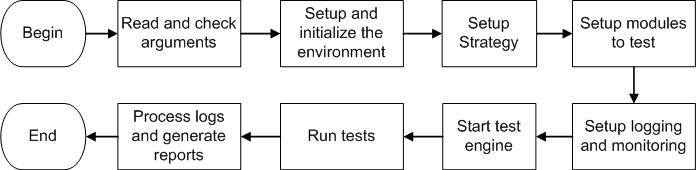
\includegraphics[width=14.5cm, height=3.5cm]{chapter3/yetiOverview.png}
	\caption{YETI test cycle}
	\label{fig:yetiOverview}
\end{figure}


\subsection{Main Components of YETI Tool}
YETI has been designed with an emphasis on extensibility to facilitate future growth. It is therefore divided into three main components: the core infrastructure, strategies and language-specific bindings which are loosely coupled to easily accommodate new languages, strategies and environments. The environment defines the procedure of extracting information from the meta-data of the classes under test and providing it to the core infrastructure. 

\begin{figure}[h]
	\centering
	\includegraphics[width=13cm, height=7.5cm]{yetiMainModules.png}
	\caption{YETI main modules}
	\label{fig:yetiMainModules}
\end{figure}

\subsubsection{YETI Core Infrastructure}
The core infrastructure is responsible for managing the test process and generation of reports. It depends on the following classes to achieve its task.
{\textbf{Yeti:}} It is the fist class in contact after the test command is issued by the user. It contains the main method of YETI which on execution parses the supplied command with options and execute the specific bindings to test the particular language requested in the command.
{\textbf{YetiLog:}} It is the class that facilitate printing debug and testing logs of the current test session. 
{\textbf{YetiLogProcessor:}} It is an interface for processing test logs.
{\textbf{YetiEngine:}} It is the class which make calls for a given number of time or specified amount of time in the command.
{\textbf{YetiTestManager:}} It is the class that is called by YetiEngine to make the actual calls.
{\textbf{YetiProgrammingLanguageProperties:}} It is a place holder for all language related instances during test.
{\textbf{YetiInitializer:}} It is an abstract class for test initialization.

The language modelling part includes the classes representing the meta-model of programming language. It consist of the following classes.
{\textbf{YetiVariable:}} It represents a variable in the YETI.
{\textbf{YetiType:}} It represents a data type in YETI.
{\textbf{YetiRoutine:}} It is a super class for routines, which represent functions, methods and constructors.
{\textbf{YetiModule:}} It represents a class under test which stores a list of modules.

\subsubsection{Strategy}
Strategy section contains seven different strategies and inputs to the tested methods is defined by one of the selected strategy. The strategies sub package of Yeti package consist of the following classes.
{\textbf{YetiStrategy:}} It is an abstract class which provides an interface for the strategies in YETI.
{\textbf{YetiRandomStrategy:}} It is a class which implements a simple random test strategy. It is a subclass of YetiStrategy.
{\textbf{YetiRandomPlusStrategy:}} It is a class which implements random+ strategy. It is an extended class of YetiRandomStrategy.
{\textbf{DSSRStrategy:}} It is a class which implements the Dirt Spot Sweeping Random strategy. It is an extended class of YetiRandomPlusStrategy.
{\textbf{ADFDStrategy:}} It is a class which implements the Automated Discovery of Failure Domain strategy. It is also an extended class of YetiRandomPlusStrategy.
{\textbf{Yeti:}}
\subsubsection{language-specific bindings}
This section can host multiple languages to enable YETI to test programs written in multiple languages. The following steps are needed to add test support for new language program in YETI. 

\begin{enumerate}
\item Define a new environment sub package in the main Yeti package such that all the related classes are contained in that environment (yeti.environment.nameOfLanguage).
\item Define a new subclass of YetiProgrammingLanguageProperties class to contain helper classes for the new language.
\item Define a new subclass of YetiInitializer to initialize the program. It is also used to read all the reflexive information about the system.
\item Define a new subclass of YetiTestManager to communicate with the target language and proceed with the actual calls.
\item Define a new subclass of YetiRoutine to actually store the definition of routines in the target language.
\item Define a new subclass of YetiModule to handle the type of modules to test.
\end{enumerate}

% if java binding example is required or instead of adding new steps if you want to show only java binding then for material check the msc thesis page 40 of test c code with Yeti.

\subsection{Construction of Test Cases}
YETI construct test cases by creating objects of the classes under test and randomly calling its methods with random inputs according to its parameter's-space. YETI split input values into two types i.e. primitive data types and user defined classes. For Java primitive data types, which includes short, byte, char, int, float, double, long etc., YETI, in its simplest random strategy, calls {\it Math.random()} method to generate an arithmetic value which is converted to the required type using casting rule of Java language. However, if the method under test needs an object of a user-defined class as a parameter then YETI calls its constructor or method to generate object of that class at run time. It may be possible that the constructor require another object and in that case YETI will recursively calls the constructor of that object. This process is continued until an object with blank constructor, constructor with only primitive types or the set level of recursion is reached.


\subsection{Command-line Options}
While YETI GUI launcher has been developed during this research study, to take maximum benefit of the available options one still need to launch YETI from CLI mode. These command-line options are case insensitive and can be provided as input to the tool in CLI mode in any order. For example, to save processing power and reduce overhead for a test session, command line option -nologs can be use to bypass real-time logging. The following table \ref{table:cliOptions} describes few of the most common command-line options available in YETI. 

\begin{table}[h]
%\scriptsize
\caption{YETI command line options} % title of Table
\smallskip
\centering % used for centering table
\begin{tabular}{|l|l|} % centered columns (4 columns)
\hline

Options									&Purpose 			\\ \hline
-java										&Test programs coded in Java	 	\\ \hline
-jml										&Test programs coded in JML			\\ \hline
-dotnet									&Test programs coded in .NET		\\ \hline
-ea											&To check code assertions \\ \hline
-nTests									&\vtop{\hbox{\strut Specify number of tests after} \hbox{\strut which the test stops}}	\\ \hline
-time										&\vtop{\hbox{\strut Specify time in seconds or minutes} \hbox{\strut after which the test stops}}\\ \hline
-testModules						&Specify one or more modules to test 	\\ \hline
-rawlogs								&Prints real time logs during test \\ \hline
-nologs									&Omit real time logs and print end result only\\ \hline
-yetiPath								&Specify path to the test modules\\ \hline
-gui										&Show test session in GUI\\ \hline
-DSSR										&\vtop{\hbox{\strut Specify Dirt Spot Sweeping Random} \hbox{\strut strategy for this session}}\\ \hline
-ADFD										&\vtop{\hbox{\strut Specify Automated Discovery of Failure} \hbox{\strut Domain strategy for this session}}\\ \hline
-random									&Specify random test strategy for this session\\ \hline
-randomPlus							&Specify random plus test strategy for this session\\ \hline
-randomPlusPeriodic			&\vtop{\hbox{\strut Specify random plus periodic test} \hbox{\strut strategy for this session}}\\ \hline
-nullProbability				&\vtop{\hbox{\strut Specify probability of inserting} \hbox{\strut null as input value}}\\ \hline
-newInstanceProability	&\vtop{\hbox{\strut Specify probability of inserting} \hbox{\strut new object as input value}}\\ \hline

\hline %inserts single line
\end{tabular}
\bigskip
\label{table:cliOptions} % is used to refer this table in the text
\end{table}


\subsection{YETI Execution}
YETI being developed in Java is highly portable and can easily run on any operating system with Java Virtual Machine (JVM) installed. YETI can be executed from both command line and GUI. To build and execute YETI, it is necessary to specify the {\it project} and all the associated {\it .jar library files} particularly {\it javassist.jar} in the {\it CLASSPATH} to help JVM in identifying the YETI source. The typical command to invoke YETI is given in figure~\ref{fig:yeticommand}. In this particular command YETI tests java.lang.String and yeti.test.YetiTest modules for 90 minutes using the default random strategy. For details of other options please see table \ref{table:cliOptions}. 

\begin{figure}[h]
	\centering
	\frame{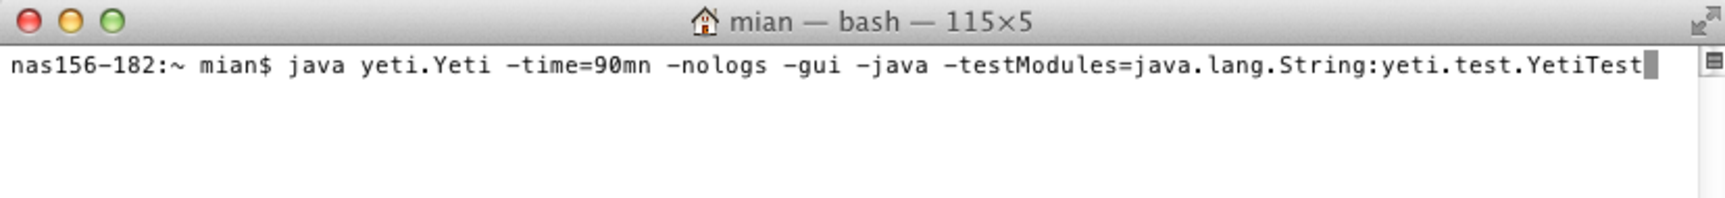
\includegraphics[width= 14cm, height = 1.8cm]{chapter3/yetiCommandCLI.pdf}}
	\caption{Command to launch YETI from CLI}
	\label{fig:yeticommand}
\end{figure}

Alternately, runnable jar file by the name {\it YetiLauncher} is also available to launch YETI from GUI. However, till the writing of this thesis, the GUI version of YETI only supports the basic options of YETI execution. Figure \ref{fig:yetiLauncher} shows the equivalent of above command in GUI mode.

\begin{figure}[h]
	\centering
	\frame{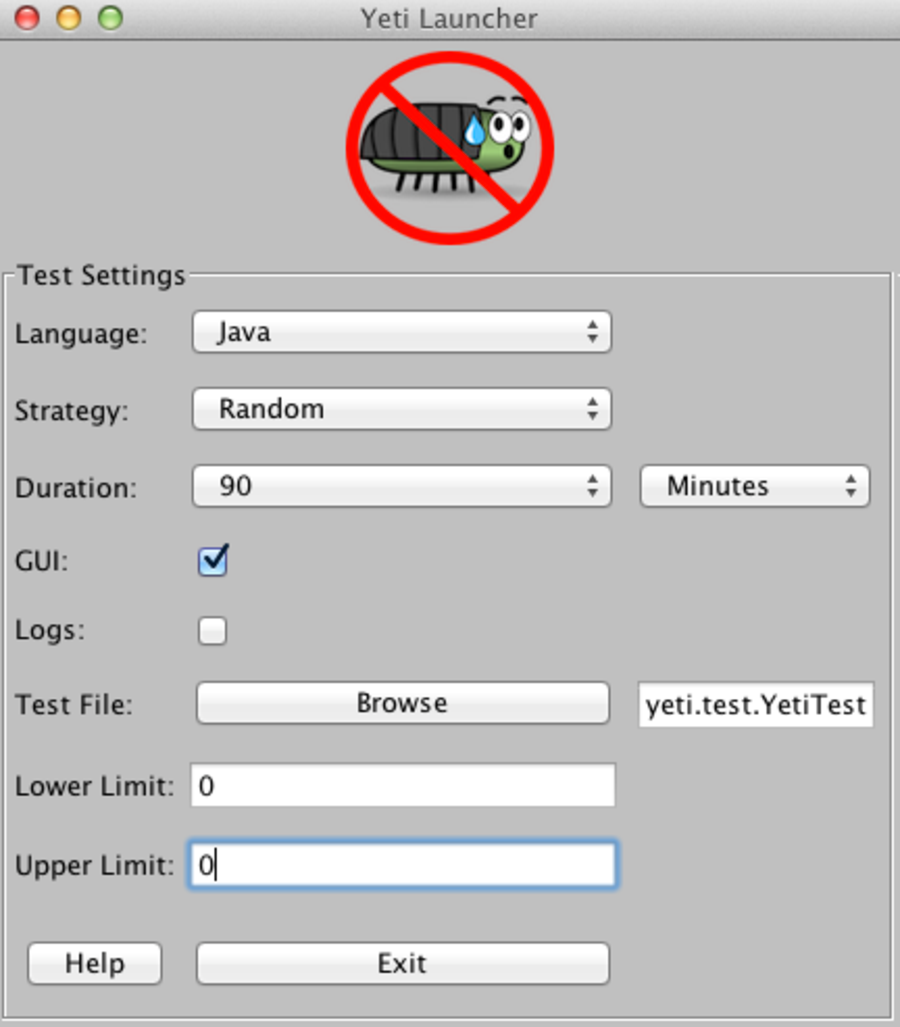
\includegraphics[width= 7cm, height = 8cm]{chapter3/yetiCommandGUI.pdf}}
	\caption{Command to launch YETI from GUI}
	\label{fig:yetiLauncher}
\end{figure}


As a result of both the above commands YETI launch its own GUI window and start testing the assigned programs. 

\subsection{YETI Test Oracle}
Oracles in YETI are language dependant. YETI uses two approaches for oracle (pass/fail judgement). In the presence of program specifications, YETI checks for inconsistencies between the code and the specifications. In the absence of specifications YETI checks for assertion violations if assert statements are included by the programmer. However in the absence of both specifications and assertions YETI performs robustness testing that considers any undeclared runtime exceptions as failures. 

%If code contracts are available, YETI uses them as oracle, however, in their absence YETI uses undeclared runtime exceptions of the underlying language as oracle. The test cases revealing errors are reproduced at the end of each test session for unit and regression testing.
%YETI deals with the oracle problem in two ways. If available, it uses code-contracts as oracles, however in the absence of contracts it uses runtime exceptions as errors which is also known as robustness testing.

\subsection{YETI Report}
YETI gives a complete test report after execution of each test. The report contain all the successful calls with the name of the routines and the unique identifiers for the parameters in each execution. These identifiers are recorded with the assign value to help in debugging the identified fault. 
\begin{figure}[h]
	\centering
	\frame{\includegraphics[width= 7cm, height = 8cm]{chapter3/seecaption.pdf}}
	\caption{YETI successful method calls}
\end{figure}

YETI separates the bugs from successful executions to simplify the test report. This approach helps debuggers to easily track the origin of the problem and rectify it. When a bug is identified during testing YETI saves that state and present it in the bug report. The information includes all the identifiers of the parameters the method call had at the time of execution. It also report the time at which the exception occurs.

\begin{figure}[h]
	\centering
	\frame{\includegraphics[width= 7cm, height = 8cm]{chapter3/seecaption.pdf}}
	\caption{YETI bug reports.}
\end{figure}

subsection{YETI Graphical User Interface}
YETI supports a GUI that not only allows test engineers to monitor the current test session but also to modify its characteristics in real time during test execution. It is useful to have the facility of modifying or aborting the test parameters at run time and observing the test behaviour in response. The figure \ref{fig:yetiGUI} present the YETI GUI comprising of six numbered windows (the windows are labelled for illustration purposes only).

\begin{figure}[h]
	\centering
	\frame{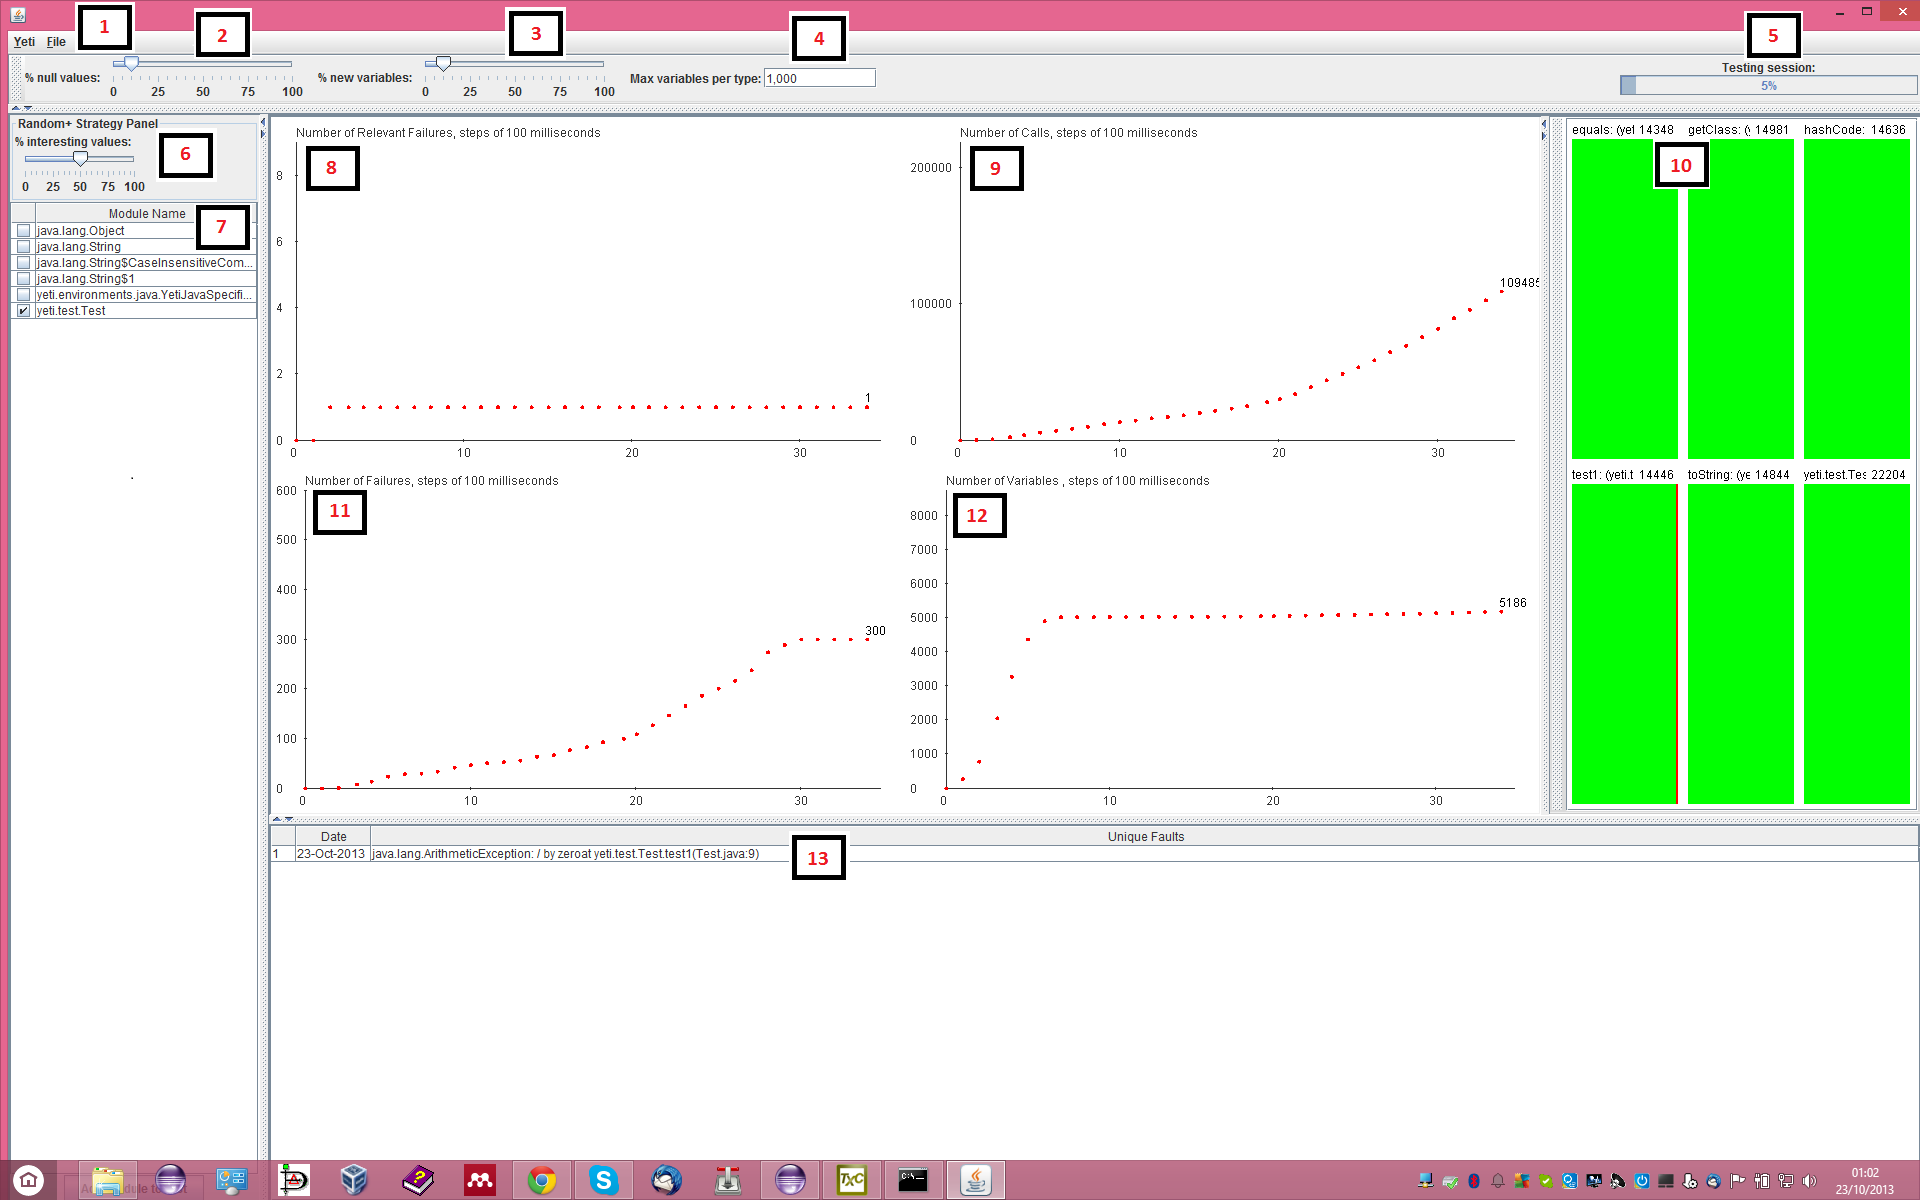
\includegraphics[width= 15cm, height = 12cm]{chapter3/yetiGUI.png}}
	\label{fig:yetiGUI}
	\caption{GUI of YETI Tool}
\end{figure}

\begin{enumerate}
\item Window No 1 displays the failures of the tested module over time.
\item Window No 2 displays the total number of failures over time. These may be generated from calls not related to the tested module.
\item Window No 3 displays the total number of calls to the tested module over time. 
\item Window No 4 displays the total number of variables generated by YETI over time.
\item Window No 5 displays colored rectangles: one for each constructor and method under test. Each rectangle represents the calls to a constructor or a method.
\item The colors in a rectangle have the following meaning:
\item Green indicates successful calls (✓). A successful call is one that does not raise an exception or if it does, the method or the constructor declares to throw it.
\item Red indicates failed calls (X). A failed call results from raised RuntimeException or one of its subclasses.
\item Yellow indicates “undecidable” calls (?). A call is “undecidable” if for some reason it takes too long to complete and needs to be stopped, or if a YetiSecurityException (custom exception in YETI) is thrown.
\end{enumerate}


\subsection{Summary of automated testing tools}

\begin{sidewaystable}
    \centering
    \caption{Summary of automated testing tools}
   \begin{tabular}{|l|l|l|l|l|l|l|}
\hline

Tool 				& Language																								& Input  																																			& Strategy 																																											 				& Output		  																								& Benefits																															& Limitations		\\ \hline
JCrasher	  & Java, JML																								& Program																																			& \vtop{\hbox{\strut Method type to predict input,}\hbox{\strut Randomly find values of crash}}  				& TC																													& \vtop{\hbox{\strut Automated TC, Use} \hbox{of Heuristic Rules}} 			& \\ \hline
Jartege			& Java																										& Classes																																			& \vtop{\hbox{\strut Random strategy with controls}\hbox{\strut like weight etc.}} 							 				& TC, RT 																											& Quick, automated																											& \\ \hline
Eclat				& Java																										& Classes, pass TC 																														& \vtop{\hbox{\strut Create model from TC, execute}\hbox{\strut each candidate on the model}} 					& Faulty TC 																									& \vtop{\hbox{\strut produce output text,} \hbox{JML}}									& \\ \hline
Quickcheck	& Haskell																									&	\vtop{\hbox{\strut Specifications}  \hbox{\strut and Functions}}	  			  & \vtop{\hbox{\strut Specification} \hbox{\strut hold to random TC?}} 											 						& Pass/Fail																										& \vtop{\hbox{\strut Easy to use, program} \hbox{documentation}}				&	\\ \hline
Randoop 		& Java, .NET																							& \vtop{\hbox{\strut Specifications,} \hbox{\strut code and time}}					  & \vtop{\hbox{\strut Generate and execute methods} \hbox{\strut \& give feedback for next generation}} 	& Fault TC, RT 																								& 																																			&	\\ \hline
AgitarOne		& Java																										& \vtop{\hbox{\strut Package, time}   \hbox{\strut and manual TC}}						& \vtop{\hbox{\strut Analyse SUT with auto and} \hbox{\strut provided data in specified time}} 					& TC, RT																											& \vtop{\hbox{\strut Eclipse plug-in} \hbox{\& easy to use}}  					& \\ \hline
AutoTest		& Java																										& \vtop{\hbox{\strut Classes, time}   \hbox{\strut and manual TC}} 						& \vtop{\hbox{\strut Heuristic rules} \hbox{\strut to evaluate contracts}} 															& violations, RT 																							& \vtop{\hbox{\strut GUI in HTML,} \hbox{easy to use}} 									& \\ \hline
TestEra			& Java																										& \vtop{\hbox{\strut Specifications,} \hbox{\strut integer \& manual TC}}			& \vtop{\hbox{\strut Check contracts} \hbox{\strut with specifications}} 																& Contracts violations 																				& \vtop{\hbox{\strut short report with} \hbox{faulty TC only}} 					& \\ \hline
Korat 			& Java																										& \vtop{\hbox{\strut Specifications}  \hbox{\strut and manual tests}}					& \vtop{\hbox{\strut Check contracts} \hbox{\strut with specifications}}																& Contracts violations 																				& \vtop{\hbox{\strut GUI, short report} \hbox{with faulty TC only}} 		& \\ \hline
YETI 				& \vtop{\hbox{\strut Java, .NET,}  \hbox{\strut JML}} 		& Code, Time 																																  & RandomPlus, Random 																																										& \vtop{\hbox{\strut Traces of found } \hbox{\strut faults}}	& \vtop{\hbox{\strut GUI, give faulty} \hbox{examples, Quick}} 				& \\ \hline %inserts single line
\end{tabular}
\label{table:Tools}
\end{sidewaystable}


%\begin{figure}[h]
%	\centering
%	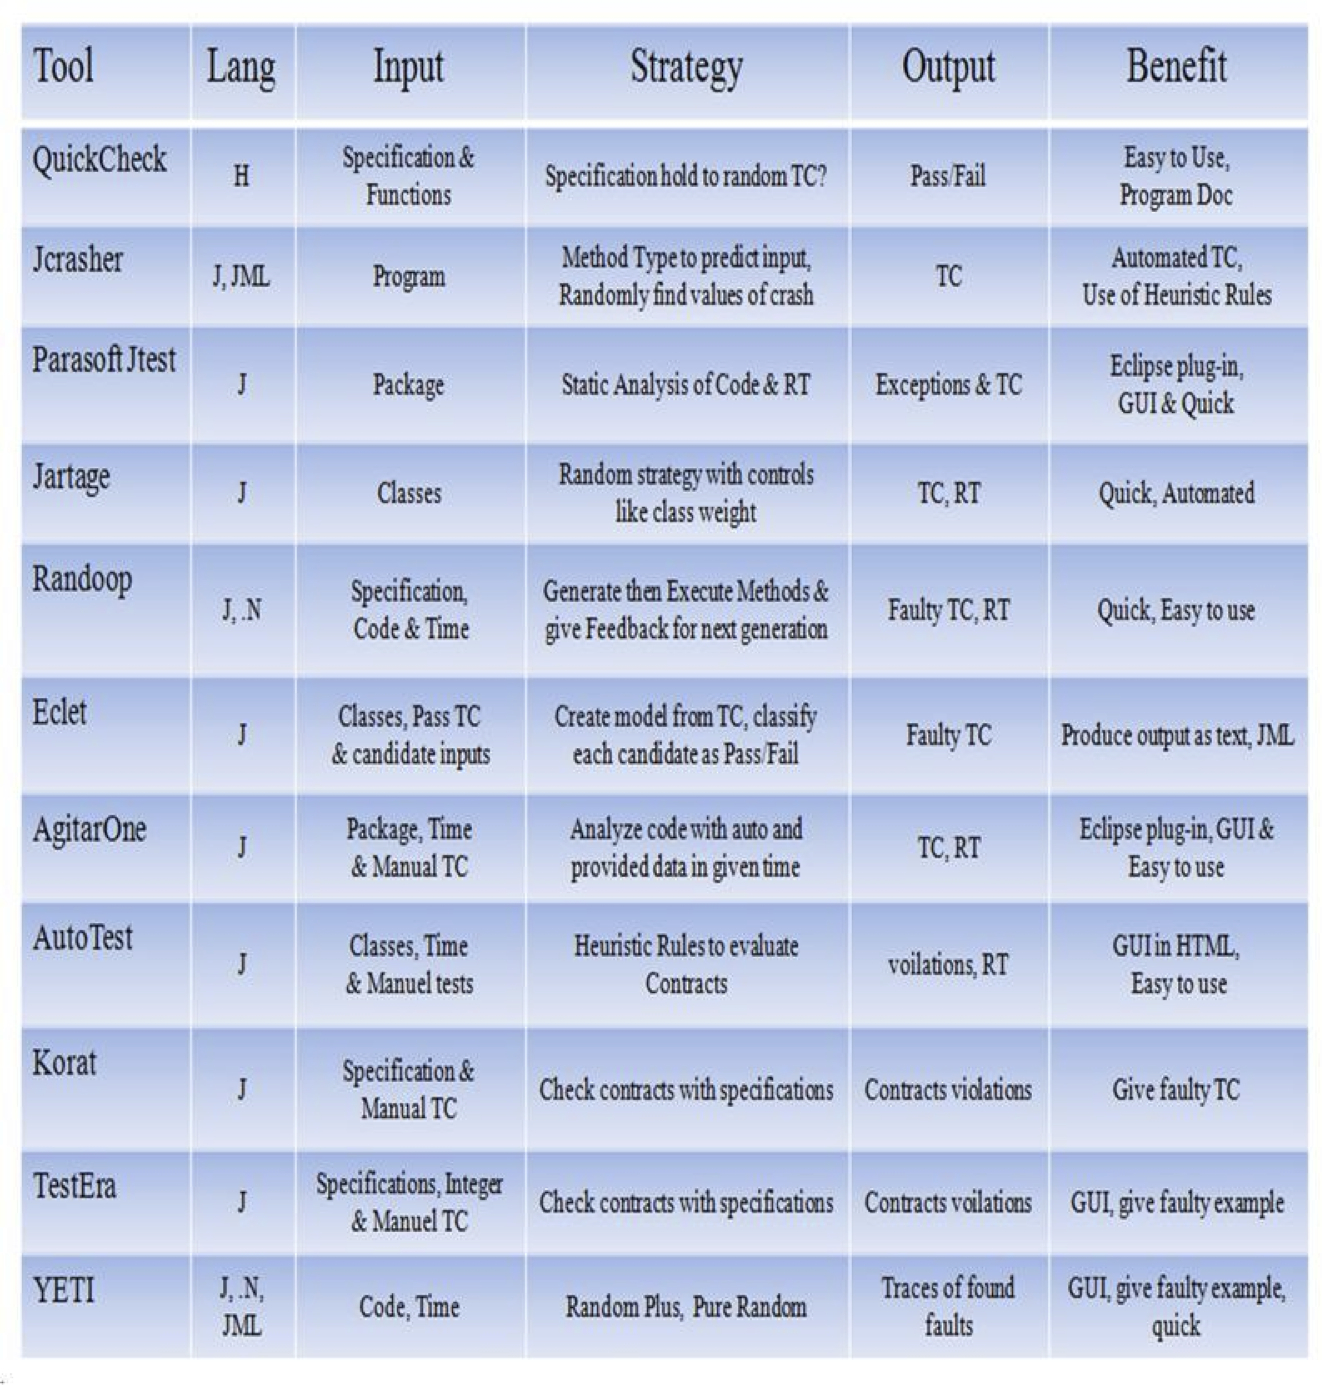
\includegraphics[scale=0.6]{chapter2/tools.jpg}
%	\caption{Summary of automated testing tools}
%\end{figure}


\section{Conclusion}


% ------------------------------------------------------------------------


%%% Local Variables:
%%% mode: latex
%%% TeX-master: "../thesis"
%%% End:
